\documentclass{article}
\usepackage{amsmath}
\usepackage{amssymb}
\usepackage{graphicx}
\usepackage{hyperref}
\usepackage[version=4]{mhchem}

\title{Problem 4}
\date{}

\begin{document}
\maketitle

\section*{Problem}
As shown in the figure, \(B D\) is a median of triangle \(A B C\). \(E\) is a point on \(A B\) such that \(C E\) bisects \(B D\) at \(F\). Find \(A B\) if \(B E=7\).\\
(A) 14\\
(B) 22\\
(C) 21\\
(D) 24\\
(E) 25\\
\centering
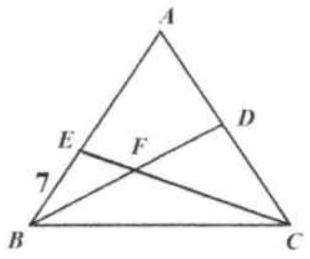
\includegraphics[width=\textwidth]{images/126(1).jpg}

\section*{Solution}
(C).\\
Method 1:\\
Pick up a point \(G\) on \(C F\) such that \(E F=F G\). Connect \(E D\), \(G D\), and \(B G\). Since the two diagonals of the quadrilateral \(B G D E\) bisect each other, \(B G D E\) is a parallelogram. It\\
\centering
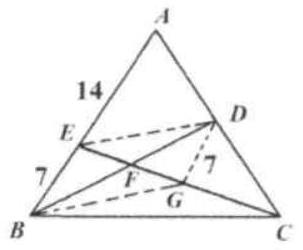
\includegraphics[width=\textwidth]{images/132(2).jpg}


follows that \(D G / / B E / / A B\). Since \(D\) is the midpoint of \(A C, G\) is the midpoint of \(C E\). So \(D G=7, A E=2 \times 7=14 . A B=7+14=21\).

Method 2:\\
Draw a parallel line to \(A B\) through \(D\) to meet \(E C\) at G . \(\triangle B E F\) is congruent to \(\triangle D G F(\angle E B F=\angle F D G, \angle E F B=\) \(\angle D F G, B F=F D\) ).\\
So \(\mathrm{DG}=\mathrm{BE}=7\). Since \(D G / / B E / / A B\) and \(D\) is the\\
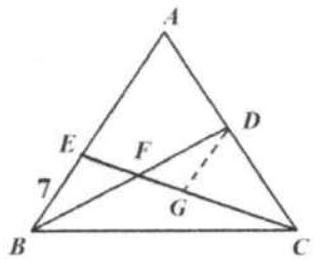
\includegraphics[width=\textwidth]{images/133.jpg} midpoint of \(A C, G\) is the midpoint of \(C E\). So \(2 D G=A E\). \(A E=2 \times 7=14 . A B=7+14=21\).

\end{document}
